\documentclass[12pt, a4paper, oneside]{ctexbook}
\usepackage{amsmath, amsthm, amssymb, bm, graphicx, hyperref, mathrsfs, float}
\usepackage{ctex}

\title{{\Huge{\textbf{那些我曾经懂过的问题}}}\\}
\author{Salieri}
\date{\today}
\linespread{1.5}
\newtheorem{theorem}{定理}[section]
\newtheorem{definition}[theorem]{定义}
\newtheorem{lemma}[theorem]{引理}
\newtheorem{corollary}[theorem]{推论}
\newtheorem{example}[theorem]{例}
\newtheorem{proposition}[theorem]{命题}
\setcounter{tocdepth}{1}%目录显示到第一级,section
\setcounter{secnumdepth}{2}%编号到第二级,subsection
\def\mt{\mathscr{T}}
\def\ms{\mathscr{S}}
\def\mf{\mathscr{F}}
\def\ml{\mathscr{L}}
\def\R{\mathbb{R}}
\def\de{definition}
\def\th{theorem}
\def\gm{$ \gamma $矩阵 }
\def\hf{Helmholtz自由能}
\def\gf{Gibbs自由能}
\newcommand{\fp}[2]{\frac{\partial#1}{\partial#2}}
\begin{document}
	\maketitle
	
	\pagenumbering{roman}
	\setcounter{page}{1}
	
	\begin{center}
		\Huge\textbf{前言}
	\end{center}~\
	
	此笔记总结我在学习过程中遇到的各种细节问题。
	~\\
	\begin{flushright}
		\begin{tabular}{c}
			Salieri\\
			\today
		\end{tabular}
	\end{flushright}
	
	\newpage
	\pagenumbering{Roman}
	\setcounter{page}{1}
	\tableofcontents
	\newpage
	\setcounter{page}{1}
	\pagenumbering{arabic}
	\chapter{凝聚态场论、量子多体}
	\section{平均场近似,高斯近似,鞍点近似,Product State}
    \section{电、声子有效相互作用}
	\section{Goldstone定理(经典)}
	考虑一个理论涉及若干个场$ \phi^a(x) $,具有如下形式的拉氏量:
	\begin{equation}
		\mathcal{L}=(\text { terms with derivatives })-V(\phi)
	\end{equation}
	令$ \phi^0_a $为最小化V的恒定场,即
	\begin{equation*}
		\left.\frac{\partial}{\partial \phi^a} V\right|_{\phi^a(x)=\phi_0^a}=0 .
	\end{equation*} 
	将V在极小值附近展开,有:
	\begin{equation*}
		V(\phi)=V\left(\phi_0\right)+\frac{1}{2}\left(\phi-\phi_0\right)^a\left(\phi-\phi_0\right)^b\left(\frac{\partial^2}{\partial \phi^a \partial \phi^b} V\right)_{\phi_0}+\cdots .
	\end{equation*}
	定义取二次项的系数作为矩阵,由于是在极小值展开,矩阵是半正定的,本征值就是质量。下面开始正式证明Goldstone定理。
	考虑某一般的连续对称变换:
	\begin{equation}
		\phi^a \longrightarrow \phi^a+\alpha \Delta^a(\phi)
	\end{equation}
	$ \alpha $是无限小参数,$ \Delta^a $是一个关于所有场的函数。考虑退化到恒定场的情况,此时含导数项自动为零,因此势能本身就需要不变,即
	\begin{equation*}
		\Delta^a(\phi) \frac{\partial}{\partial \phi^a} V(\phi)=0
	\end{equation*} 
	此式再对$ \phi^b $求导,并取$ \phi=\phi_0 $:
	\begin{equation*}
		0=\left(\frac{\partial \Delta^a}{\partial \phi^b}\right)_{\phi_0}\left(\frac{\partial V}{\partial \phi^a}\right)_{\phi_0}+\Delta^a\left(\phi_0\right)\left(\frac{\partial^2}{\partial \phi^a \partial \phi^b} V\right)_{\phi_0}
	\end{equation*}   
	由于$ \phi_0 $使得V最小,第一项自动为0,因此第二项也等于零。若对称性依然对于场$ \phi_0 $成立,$ \Delta^a(\phi_0)=0 $。若发生自发对称性破缺,则二阶导项为零,即质量为零。   
    \chapter{量子信息}
    \section{Multipartite Entanglement}
	\chapter{量子场论}
    \section{同一粒子的不同表示}
	\section{Dirac,Weyl and Majorana fermions}\cite{pal2011dirac}
	简单来讲,Dirac fermion是Dirac方程的一般解,Majorana fermion是Dirac方程的“实”解,Weyl fermion是无质量Dirac方程的解。\\
	\subsection{Dirac方程及其解}
	Dirac方程定义为:
	\begin{equation}
		\left(i \gamma^\mu \partial_\mu-m\right) \Psi=0\label{de}
	\end{equation}
	它可以看作具有如下哈密顿量的薛定谔方程:
	\begin{equation}
		H=\gamma^0\left(\gamma^i p^i+m\right)
	\end{equation}
	$\gamma$ 矩阵定义为:
	\begin{equation}
		\begin{aligned}
			& {\left[\gamma^\mu, \gamma^\nu\right]_{+}=2 g^{\mu \nu},} \\
			& \gamma_0 \gamma_\mu \gamma_0=\gamma_\mu^{\dagger}
			\end{aligned}
	\end{equation}
	可以看到,当$ \gamma $矩阵为纯虚时,Dirac方程为实方程,有实解。我们可以找到一组\gm 满足这样的条件,这个表象称为Majorana表象。
	\begin{equation}
		\begin{array}{ll}
			\widetilde{\gamma}^0=\left[\begin{array}{cc}
			0 & \sigma^2 \\
			\sigma^2 & 0
			\end{array}\right], \quad \widetilde{\gamma}^1=\left[\begin{array}{cc}
			i \sigma^1 & 0 \\
			0 & i \sigma^1
			\end{array}\right], \\
			\tilde{\gamma}^2=\left[\begin{array}{cc}
			0 & \sigma^2 \\
			-\sigma^2 & 0
			\end{array}\right], \quad \tilde{\gamma}^3=\left[\begin{array}{cc}
			i \sigma^3 & 0 \\
			0 & i \sigma^3
			\end{array}\right],
			\end{array}
	\end{equation}
	其中$ \sigma^i $为Pauli矩阵。在此表象下写出Dirac方程,我们有实解:
	\begin{equation}
		\widetilde{\psi}=\tilde{\psi}^{\star}\label{rc}
	\end{equation} 
	此解即代表Majorana fermion。\gm 不同表示之间通过幺正变换相联系:
	\begin{equation}
		\gamma^\mu=U \tilde{\gamma}^\mu U^{\dagger}
	\end{equation}
	此时解$ \tilde{\Psi} $与Majorana表象下的解也通过一个幺正矩阵相联系:
	\begin{equation}
		\Psi=U \tilde{\Psi}
	\end{equation} 
	实解条件\eqref{rc}此时为
	\begin{equation}
		\psi=U U^{\top} \psi^{\star}
	\end{equation}
	我们一般不直接使用幺正矩阵$ U $,而是转而定义如下矩阵:
	\begin{equation}
		U U^{\top}=\gamma_0 C
	\end{equation} 
	由此定义协变共轭(协变性将在稍后证明):
	\begin{equation}
		\hat{\Psi} \equiv \gamma_0 C \Psi^{\star}\label{ccg}
	\end{equation}
	此时实解条件\eqref{rc}可以写为:
	\begin{equation}
		\hat{\psi}=\psi\label{grc}
	\end{equation}
	\subsection{Fourier展开}
	一个Majorana fermion解在一般的表象下的Fourier展开为:
	\begin{equation}
		\psi(x)=\sum_s \int_p\left(a_s(p) u_s(p) e^{-i p \cdot x}+a_s^{\dagger}(p) v_s(p) e^{+i p \cdot x}\right)
	\end{equation}
	v和u互为协变共轭$ v_s(p)=\gamma_0 C u_s^{\star}(p) $
	\subsection{矩阵C的一些性质}
	除了通过找到实解对应的Majorana表象外,我们还可以通过研究 C矩阵本身的性质来定义一组C矩阵,再由此找到不依赖于表象的“实解”条件。\\
	简单观察可以发现,C矩阵满足如下性质:
	\begin{equation}
		C^{-1} \gamma_\mu C=-\left(U \tilde{\gamma}_\mu U^{\dagger}\right)^{\top}=-\gamma_\mu^{\top}
	\end{equation} 
	事实上,对于任何表象的\gm 我们总可以找到满足上式的C矩阵,此式可以直接称为C矩阵的定义,由此我们有一般情况的实解条件\eqref{grc}
    同时,很容易验证C矩阵在任意表象下都是完全反对称矩阵。
	\subsection{实条件的洛伦兹不变性}
	此节将阐述为什么称\eqref{ccg}为协变共轭,我们取Lorentz变换的生成元为$ \sigma^{\mu\nu}=\frac{i}{2}[\gamma_\mu,\gamma_\nu]  $,注意,这并非Pauli矩阵。一个fermion场的变换为:
	\begin{equation}
		\Psi^{\prime}\left(x^{\prime}\right)=\exp \left(-\frac{i}{4} \omega^{\mu \nu} \sigma_{\mu \nu}\right) \Psi(x)
	\end{equation}
	对上式取复共轭并左乘$ \gamma_0C $,注意到\gm 的性质,可以推出:
	\begin{equation}
		\widehat{\Psi}^{\prime}\left(x^{\prime}\right)=\exp \left(-\frac{i}{4} \omega^{\mu \nu} \sigma_{\mu \nu}\right) \widehat{\Psi}(x)
	\end{equation} 
	由此可以看出,协变共轭场于原场具有相同的洛伦兹变换规则,所以实解条件是洛伦兹不变的。
	\subsection{左与右}
	在处理费米场时,我们通常会遇到两个和左右有关的概念,螺旋度(helicity)和手性(chirality),两者通常并不相同,但在某些情况下又有关联,本节将阐述这种关联。
	\paragraph*{螺旋度}
	满足Dirac方程的费米子额度螺旋度定义为:
	\begin{equation}
		h_p=\frac{\boldsymbol{\Sigma} \cdot \boldsymbol{p}}{\mathrm{p}}
	\end{equation}
	$ \boldsymbol{\Sigma} $为自旋矩阵。很显然,$ h_p $的本征值为$ \pm $  1,分别对应“右手”和“左手”。可以验证  $ h_p $与哈密顿量对易,也就是说它是一个守恒量,并且其点乘结构也保证了旋转不变形,但可以验证对于有质量粒子,螺旋度在推动下是改变的。
	一个简单的论证是考虑螺旋度的物理意义:自旋在动量方向上的投影,考虑在粒子速度方向上一运动更快的参考系,此时动量反号,但自旋投影在该boost下不改变,因此螺旋度改变。
	上面的论述依赖于速度更快的参考系,这对无质量粒子是不可能的,因此这暗示无质量粒子的螺旋度是一个真正的洛伦兹不变量。
	\paragraph*{手性}
	可以额外定义一个矩阵$ \gamma_5 $,它满足:
	\begin{equation}
		\left[\gamma_5, \gamma_\mu\right]_{+}=0 \quad \forall \mu
	\end{equation} 
	一个显然的解是:
	\begin{equation}
		\gamma_5=i \gamma^0 \gamma^1 \gamma^2 \gamma^3
	\end{equation}
	给上式乘上额外的相因子也是满足定义的,上述的选择保证了$ \gamma_5 $有如下性质:
	\begin{equation}
		\gamma_5^{\dagger}=\gamma_5, \quad\left(\gamma_5\right)^2=1
	\end{equation} 
	后者保证了如下定义的两个矩阵确实是投影算符:
	\begin{equation}
		L=\frac{1}{2}\left(1-\gamma_5\right), \quad R=\frac{1}{2}\left(1+\gamma_5\right)
	\end{equation}
	两者的本征空间里的矢量分别称为“左手”的和“右手”的。每个Dirac旋量也总可以拆分成两者之和。可以验证,$ \gamma_5 $与洛伦兹变换的生成元对易,但与哈密顿量不对易,这是由于质量相含一个\gm ,因此和$ \gamma_5 $反对易。
	\subsection{Wyle fermion}
	如前文所述,质量项同时阻碍了螺旋度和手性成为性质良好的物理量,因此我们考虑无质量费米子。由于$ \gamma_5 $的存在以及Schur引理,
	一般的Dirac方程解并非Lorentz群的不可约表示,而手性解是可约的,称为Wyle fermion。一个一般的费米子是可约表示$ \frac{1}{2}\oplus\frac{1}{2} $,
	即一个左手Wyle一个右手Wyle。上述说法对螺旋度同样适用,因为无质量时两者相同。
	\subsection{从Wyle费米子到Majorana 与Dirac费米子}
	Majorana fermion是含有质量的,因此必须包含左右手两部分,考虑到实条件,这必须是一个Wyle场与它的协变共轭:
	\begin{equation}
		\psi(x)=\chi(x)+\widehat{\chi}(x)
	\end{equation}
	而Dirac fermion的区别就是没有实解条件,因此两个左手、右手场之间独立:
	\begin{equation}
		\Psi(x)=\chi_1(x)+\widehat{\chi}_2(x)
	\end{equation}
	\section{Pology}
	\section{Noether定理与local对称性}
    \section{规范场的量子化:QED,非阿贝尔,与凝聚态中的电磁场路径积分}
	\section{外场与有效作用量}
	\subsection{来自热力学的类比}
	考虑一个磁性系统,配分函数以及Helmholtz自由能为:
	\begin{equation}
		Z(H)=e^{-\beta F(H)}=\int \mathcal{D} s \exp \left[-\beta \int d x(\mathcal{H}[s]-H s(x))\right]
	\end{equation}
	$ H $为外加磁场。磁化强度可以通过对Helmholtz自由能求导得到:
	\begin{equation*}
		\begin{aligned}
			-\left.\frac{\partial F}{\partial H}\right|_{\beta \text { fixed }} & =\frac{1}{\beta} \frac{\partial}{\partial H} \log Z \\
			& =\frac{1}{Z} \int d x \int \mathcal{D} s s(x) \exp \left[-\beta \int d x(\mathcal{H}[s]-H s)\right] \\
			& =\int d x\langle s(x)\rangle \equiv M .
			\end{aligned}
	\end{equation*}
	\gf 通过Legendre变换得到
	\begin{equation*}
		G=f+MH
	\end{equation*}
	外场可以对\gf 求导得到:
	\begin{equation}
		\begin{aligned}
			\frac{\partial G}{\partial M} & =\frac{\partial F}{\partial M}+M \frac{\partial H}{\partial M}+H \\
			& =\frac{\partial H}{\partial M} \frac{\partial F}{\partial H}+M \frac{\partial H}{\partial M}+H \\
			& =H
			\end{aligned}
	\end{equation}
	当$ H=0 $时,\gf 取极值,热力学上最稳定的态由$ G(M) $的最小值给出。通过类比,我们也可以在QFT中构造相似的量,为方便仅考虑标量场。
	\subsection{有效作用量的引入}
	 标量场的生成函数为:
	 \begin{equation}
		Z[J]=e^{-i E[J]}=\int \mathcal{D} \phi \exp \left[i \int d^4 x(\mathcal{L}[\phi]+J \phi)\right]
	 \end{equation}
	 一般而言通常的记号并非$ E(J) $,而是$ W(J) $,后文中可能交替使用两种记号。可以看出$ E(J) $可以类比\hf ,它的物理意义是
	 真空-真空振幅的联通部分。J类比外磁场。之后的讨论中我们假定J是均匀的,通过泛函的一些技巧我们很容易推广到一般的场。\\
	 令$ E(J) $对J求泛函导数,有:
	 \begin{equation}
		\frac{\delta}{\delta J(x)} E[J]=i \frac{\delta}{\delta J(x)} \log Z=-\frac{\int \mathcal{D} \phi e^{i \int(\mathcal{L}+J \phi)} \phi(x)}{\int \mathcal{D} \phi e^{i \int(\mathcal{L}+J \phi)}}
	 \end{equation}  
	将上式简记为:
	\begin{equation}
		\frac{\delta}{\delta J(x)} E[J]=-\langle\Omega|\phi(x)| \Omega\rangle_J
	\end{equation}
	等式右侧为有场J时$ \phi $的真空期望。注意到热力学中和外场共轭的物理量也是内场的平均值,因此我们定义:
	\begin{equation}
		\phi_{\mathrm{cl}}(x)=\langle\Omega|\phi(x)| \Omega\rangle_J
		\label{defofcf}
	\end{equation}
	由此定义\gf 的QFT类比,即$ E(J) $的Legendre变换:\\
	(note:在Weinberg等教材中,此处的Legendre变换定义略有不同,并没有取场在源J的真空期望值作为Legendre变换中和J共轭的量
	,而是定义$ J_{\phi 人} $为产生期望值为$ \phi^r $的流,再定义Legendre变换:
	\begin{equation}
		\Gamma[\phi] \equiv-\int \mathrm{d}^4 x \phi^r(x) J_{\phi r}(x)+W\left[J_\phi\right]
		\label{defofw}
	\end{equation}  
	后文在计算有效作用量时主要采用了这个定义)
	\begin{equation}
		\Gamma\left[\phi_{\mathrm{cl}}\right] \equiv-E[J]-\int d^4 y J(y) \phi_{\mathrm{cl}}(y)
		\label{defofea}
	\end{equation} 
	对经典场再求泛函导数,有:
	\begin{equation}
		\begin{aligned}
			\frac{\delta}{\delta \phi_{\mathrm{cl}}(x)} \Gamma\left[\phi_{\mathrm{cl}}\right] & =-\frac{\delta}{\delta \phi_{\mathrm{cl}}(x)} E[J]-\int d^4 y \frac{\delta J(y)}{\delta \phi_{\mathrm{cl}}(x)} \phi_{\mathrm{cl}}(y)-J(x) \\
			& =-\int d^4 y \frac{\delta J(y)}{\delta \phi_{\mathrm{cl}}(x)} \frac{\delta E[J]}{\delta J(y)}-\int d^4 y \frac{\delta J(y)}{\delta \phi_{\mathrm{cl}}(x)} \phi_{\mathrm{cl}}(y)-J(x) \\
			& =-J(x) .
			\end{aligned}
	\end{equation}
	热力学和QFT的类比总结如图\ref*{Analog}:\\
	\begin{figure}[htp]
		\centering
		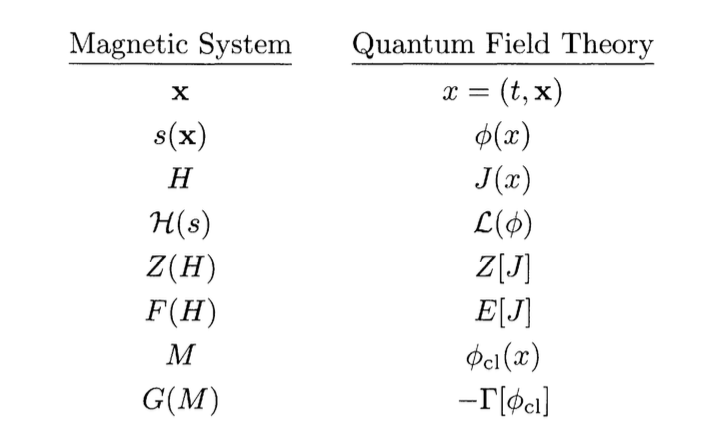
\includegraphics[scale=0.8]{analog.png}
		\caption{热力学与QFT类比}
		\label{Analog}
	\end{figure}
	很容易看出,当外场为零时,有:
	\begin{equation}
		\frac{\delta}{\delta \phi_{\mathrm{cl}}(x)} \Gamma\left[\phi_{\mathrm{cl}}\right]=0
		\label{ec}
	\end{equation}
	此方程的解就是理论中的稳定构型。对于平移不变的真空态,解是不依赖于x的,但有时也会有额外的解称为瞬子。\\
	在此假设考虑的理论中可能的真空态在平移以及Lorentz变换下总是不变的,此时方程变为非常简单的非泛函方程,进一步我们知道
	$ \Gamma $是一个广延量,它正比于我们所选取的时空体积:
	\begin{equation}
		\Gamma\left[\phi_{\mathrm{cl}}\right]=-(V T) \cdot V_{\mathrm{eff}}\left(\phi_{\mathrm{cl}}\right)
	\end{equation} 
	系数$ V_{\mathrm{eff}}\left(\phi_{\mathrm{cl}}\right) $称为有效势。$ \Gamma\left[\phi_{\mathrm{cl}}\right] $
	取极值的条件简化为$ V_{\mathrm{eff}}\left(\phi_{\mathrm{cl}}\right) $取极值。
	\subsection{有效作用量的性质}
	先给出结论:我们知道$ Z[J] $是关联函数的生成泛函,而$ \Gamma\left[\phi_{\mathrm{cl}}\right] $ 是单粒子不可约关联函数
	的生成泛函。为看出这一点,从两点关联函数算起。
	\begin{equation}
		\begin{aligned}
			& \frac{\delta^2 E[J]}{\delta J(x) \delta J(y)}=-\frac{i}{Z} \int \mathcal{D} \phi e^{i \int(\mathcal{L}+J \phi)} \phi(x) \phi(y) \\
			& \quad+\frac{i}{Z^2} \int \mathcal{D} \phi e^{i \int(\mathcal{L}+J \phi)} \phi(x) \cdot \int \mathcal{D} \phi e^{i \int(\mathcal{L}+J \phi)} \phi(y) \\
			&=-i[\langle\phi(x) \phi(y)\rangle-\langle\phi(x)\rangle\langle\phi(y)\rangle] .
			\end{aligned}
	\end{equation}
	 非连通部分刚好被抵消,对更高阶的泛函导数也有相同的结果(link cluster theorem),因此有:
	 \begin{equation}
		\frac{\delta^n E[J]}{\delta J\left(x_1\right) \cdots \delta J\left(x_n\right)}=(i)^{n+1}\left\langle\phi\left(x_1\right) \cdots \phi\left(x_n\right)\right\rangle_{\mathrm{conn}}
	 \end{equation}
	 现在开始考虑$ \gamma $,对\eqref{ec}求场$ J(y) $的泛函导数有:
	 \begin{equation*}
		\frac{\delta}{\delta J(y)} \frac{\delta \Gamma}{\delta \phi_{\mathrm{cl}}(x)}=-\delta(x-y)
	 \end{equation*} 
	 利用链式法则展开左式:
	 \begin{equation}
		\begin{aligned}
			\delta(x-y) & =-\int d^4 z \frac{\delta \phi_{\mathrm{cl}}(z)}{\delta J(y)} \frac{\delta^2 \Gamma}{\delta \phi_{\mathrm{cl}}(z) \delta \phi_{\mathrm{cl}}(x)} \\
			& =\int d^4 z \frac{\delta^2 E}{\delta J(y) \delta J(z)} \frac{\delta^2 \Gamma}{\delta \phi_{\mathrm{cl}}(z) \delta \phi_{\mathrm{cl}}(x)} \\
			& =\left(\frac{\delta^2 E}{\delta J \delta J}\right)_{y z}\left(\frac{\delta^2 \Gamma}{\delta \phi_{\mathrm{cl}} \delta \phi_{\mathrm{cl}}}\right)_{z x}
			\end{aligned}
			\label{2p}
	 \end{equation}
	 可以看到这两个无限维矩阵互为逆:
	 \begin{equation}
		\left(\frac{\delta^2 E}{\delta J \delta J}\right)=\left(\frac{\delta^2 \Gamma}{\delta \phi_{\mathrm{cl}} \delta \phi_{\mathrm{cl}}}\right)^{-1}
	 \end{equation}
	 已知左式为连通两点关联函数,即传播子,因此右式为传播子的逆。到动量空间可以更容易看出物理意义:
	 \begin{equation*}
		\widetilde{D}^{-1}(p)=-i\left(p^2-m^2-M^2\left(p^2\right)\right)
	 \end{equation*}
	 $ M^2\left(p^2\right) $是自能函数,是所有单粒子不可约两点图的求和。进一步求泛函导数,用链式法则改写求导:
	 \begin{equation*}
		\frac{\delta}{\delta J(z)}=\int d^4 w \frac{\delta \phi_{\mathrm{cl}}(w)}{\delta J(z)} \frac{\delta}{\delta \phi_{\mathrm{cl}}(w)}=i \int d^4 w D(z, w) \frac{\delta}{\delta \phi_{\mathrm{cl}}(w)}
	 \end{equation*}
	 并利用矩阵逆求导的法则:
	 \begin{equation*}
		\frac{\partial}{\partial \alpha} M^{-1}(\alpha)=-M^{-1} \frac{\partial M}{\partial \alpha} M^{-1}
	 \end{equation*}
	 继续对\eqref{2p}求泛函导数,有:
	 \begin{equation*}
		\begin{aligned}
			\frac{\delta^3 E[J]}{\delta J_x \delta J_y \delta J_z} & =i \int d^4 w D(z, w) \frac{\delta}{\delta \phi_w^{\mathrm{cl}}}\left(\frac{\delta^2 \Gamma}{\delta \phi_x^{\mathrm{cl}} \delta \phi_y^{\mathrm{cl}}}\right)^{-1} \\
			& =i \int d^4 w D_{z w}(-1) \int d^4 u \int d^4 v\left(-i D_{x u}\right) \frac{\delta^3 \Gamma}{\delta \phi_u^{\mathrm{cl}} \delta \phi_v^{\mathrm{cl}} \delta \phi_w^{\mathrm{cl}}}\left(-i D_{v y}\right)\\
			& =i \int d^4 u d^4 v d^4 w D_{x u} D_{y v} D_{z w} \frac{\delta^3 \Gamma}{\delta \phi_u^{\mathrm{cl}} \delta \phi_v^{\mathrm{cl}} \delta \phi_w^{\mathrm{cl}}}
		\end{aligned}
	 \end{equation*}
	 \begin{figure}[htp]
		\centering
		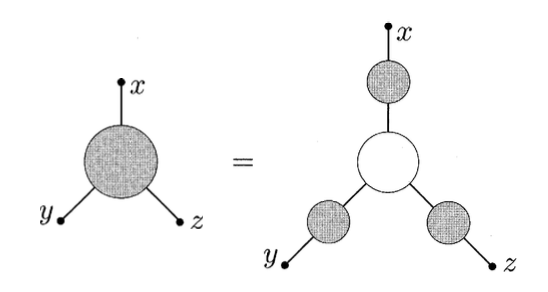
\includegraphics[scale=1]{3DR.png}
		\caption{三点关系的图像表示}
		\label{3DR}
	\end{figure}
	深灰圈表示连通图的求和,浅灰圈表示量子作用量的三阶泛函导数,可以看出它代表所有完全传播子移除后的连通三点关联函数,
	即单粒子不可约三点函数:
	\begin{equation*}
		\frac{i \delta^3 \Gamma}{\delta \phi_{\mathrm{cl}}(x) \phi_{\mathrm{cl}}(y) \phi_{\mathrm{cl}}(z)}=\langle\phi(x) \phi(y) \phi(z)\rangle_{1 \mathrm{PI}}
	\end{equation*}
	继续求导,可以总结出以下关系:
	\begin{equation}
		\frac{\delta^n \Gamma\left[\phi_{\mathrm{cl}}\right]}{\delta \phi_{\mathrm{cl}}\left(x_1\right) \cdots \delta \phi_{\mathrm{cl}}\left(x_n\right)}=-i\left\langle\phi\left(x_1\right) \cdots \phi\left(x_n\right)\right\rangle_{1 \mathrm{PI}}
	\end{equation}
	因此我们得出,量子有效作用量是单粒子不可约关联函数的生成泛函。因此,类比$ W(J) $是所有连通真空-真空图的求和,$ \Gamma[\phi_{cl}] $是所有单粒子不可约
	连通图的求和。 \\
	若将生成泛函中的经典作用量$ I[\phi] $直接换成量子有效作用量$ \Gamma[\phi] $,则有:
	\begin{equation}
		Z_{\Gamma}[j]=e^{W_{\Gamma}[j]}=\int[D \phi(x)] \exp \left[i \Gamma[\phi(x)]+i \int d^4 x j(x) \phi(x)\right]
	\end{equation}   
	我们将证明,这个生成泛函所代表的真空-真空振幅的连通树图部分给出了原本经典作用量$ I[\phi] $的理论的所有阶贡献。为分离出
	树图部分,引入一个常数试图标记不同部分的贡献:
	\begin{equation}
		Z_r[j ; \hbar]=e^{w_r[j ; \hbar]}=\int[D \phi(x)] \exp \left[\frac{i}{\hbar}\left(\Gamma[\phi(x)]+\int d^4 x j(x) \phi(x)\right)\right]
	\end{equation}
	传播子给出贡献$ \hbar $,顶点给出贡献$ \hbar^{-1} $,又拓扑恒等式,圈数$ n_L $、内线数I,顶点数V有关系$ n_L=I-V+1 $,
	因此L圈图的贡献正比于$ \hbar^{n_L-1} $,形式上可以有:
	\begin{equation}
		W_{\Gamma}[j ; \hbar]=\sum_{n_L=0}^{\infty} \hbar^{n_L-1} \underbrace{W_{\Gamma, n_L}[j]}_{n_L \text { loops }}
	\end{equation}     
	为分离出树图,形式上取极限$ \hbar\to 0 $,此时圈图贡献趋于零,且路径积分由稳相点主导。 
	\subsection{有效作用量的计算}
	我们在重整微扰论的框架下,从定义式\eqref{defofea}出发,逐阶计算泛函。首先,照常把拉氏量写为两部分:
	\begin{equation}
		\mathcal{L}=\mathcal{L}_1+\delta \mathcal{L}
	\end{equation}
	把流分为两部分$ J(x)=J_1(x)+\delta J(x) $ ,其中一部分满足如下方程:
	\begin{equation}
		\left.\frac{\delta \mathcal{L}_1}{\delta \phi}\right|_{\phi=\phi_{\mathrm{cl}}}+J_1(x)=0
		\label{defofj1}
	\end{equation}
	而$ \delta J(x) $的取值是的总的流让场的真空期望值仍是$ \phi_{cl}(x) $ 即$ \langle\phi(x)\rangle_J=\phi_{\mathrm{cl}}(x) $\\
	现在生成泛函为:
	\begin{equation}
		Z[J]=\int \mathcal{D} \phi e^{i \int d^4 x\left(\mathcal{L}_1[\phi]+J_1 \phi\right)} e^{i \int d^4 x(\delta \mathcal{L}[\phi]+\delta J \phi)}
	\end{equation}
	平移场的定义,取$ \phi(x)=\phi_{\mathrm{cl}}(x)+\eta(x) $ ,指数中的项做幂级数展开:
	\begin{equation}
		\begin{aligned}
			\int d^4 x\left(\mathcal{L}_1+J_1 \phi\right) & =\int d^4 x\left(\mathcal{L}_1\left[\phi_{\mathrm{cl}}\right]+J_1 \phi_{\mathrm{cl}}\right)+\int d^4 x \eta(x)\left(\frac{\delta \mathcal{L}_1}{\delta \phi}+J_1\right) \\
			& +\frac{1}{2} \int d^4 x d^4 y \eta(x) \eta(y) \frac{\delta^2 \mathcal{L}_1}{\delta \phi(x) \delta \phi(y)} \\
			& +\frac{1}{3 !} \int d^4 x d^4 y d^4 z \eta(x) \eta(y) \eta(z) \frac{\delta^3 \mathcal{L}_1}{\delta \phi(x) \delta \phi(y) \delta \phi(z)}+\cdots
			\end{aligned}
	\end{equation}
	一阶项由\eqref{defofj1}直接为零,二阶项给出高斯积分,高阶项视作微扰修正。暂且忽略抵消项与高阶修正,高斯积分给出有效作用量的第一个修正项:
	\begin{equation}
		\begin{aligned}
			\int \mathcal{D} \eta & \exp \left[i\left(\int\left(\mathcal{L}_1\left[\phi_{\mathrm{cl}}\right]+J_1 \phi_{\mathrm{cl}}\right)+\frac{1}{2} \int \eta \frac{\delta^2 \mathcal{L}_1}{\delta \phi \delta \phi} \eta\right)\right] \\
			= & \exp \left[i \int\left(\mathcal{L}_1\left[\phi_{\mathrm{cl}}\right]+J_1 \phi_{\mathrm{cl}}\right)\right] \cdot\left(\operatorname{det}\left[-\frac{\delta^2 \mathcal{L}_1}{\delta \phi \delta \phi}\right]\right)^{-1 / 2} .
			\end{aligned}
	\end{equation}
	高阶项的作用在Feynman图表示中,给出了一系列以$ -i\left(\frac{\delta^2 \mathcal{L}_1}{\delta \phi \delta \phi}\right)^{-1} $ 
	作为传播子,高阶项作为顶点的Feynman规则图。\\
	考虑抵消项,也在$ \phi_{cl} $处展开,有 
	\begin{equation}
		\left(\delta \mathcal{L}\left[\phi_{\mathrm{cl}}\right]+\delta J \phi_{\mathrm{cl}}\right)+\left(\delta \mathcal{L}\left[\phi_{\mathrm{cl}}+\eta\right]-\delta \mathcal{L}\left[\phi_{\mathrm{cl}}\right]+\delta J \eta\right)
	\end{equation}
	第二项Taylor展开后也给出Feynman图修正,第一项是一个常数。总结,有效作用量为:
	\begin{equation}
		\begin{aligned}
			\Gamma\left[\phi_{\mathrm{cl}}\right]= & \int d^4 x \mathcal{L}_1\left[\phi_{\mathrm{cl}}\right]+\frac{i}{2} \log \operatorname{det}\left[-\frac{\delta^2 \mathcal{L}_1}{\delta \phi \delta \phi}\right] \\
			& -i \cdot(\text { connected diagrams })+\int d^4 x \delta \mathcal{L}\left[\phi_{\mathrm{cl}}\right]
			\end{aligned}
	\end{equation}
	上述连通图都是真空-真空图,至少也是两圈图,因此最低阶修正就是泛函行列式。上面的构造中比正常的重整化多了一个抵消项:$ \delta J $,它由
	下述方法给出:\\
	首先在头阶项有关系$ \langle\phi\rangle=\phi_{\mathrm{cl}} $,此等式会因为Feynman图给出的修正而不成立,且贡献都来自于
	“蝌蚪”图,他们刚好可以由$ \delta J\eta $项抵消是的等式依然成立。在实际操纵中我们直接忽略连通单粒子不可约单点图,因为刚好被
	$ \delta J\eta $抵消。
	\subsection{有效作用量的对称性}
	虽然不总是这样, 但在某些情况下, 作用量$ I[\phi] $ 的对称性自动地也是有效作用量的$ \Gamma[\phi] $ 的对称性。除非我们能够证明附加于作用量的对称性也适用于有效作用量, 否则我们在建立理论的可重 整性时会遇到问题。\\
	为此没我们研究一种重要的对称性,它由如下无限小变换生成:
	\begin{equation}
		\chi^n(x) \rightarrow \chi^n(x)+\epsilon F^n[x ; \chi]
	\end{equation}
	假定测度和作用量在变换下都不变:
	\begin{equation}
		\begin{aligned}
			I[\chi+\epsilon F] & =I[\chi] \\
			\prod_{n, x} \mathrm{~d}\left(\chi^n(x)+\epsilon F[x ; \chi]\right) & =\prod_{n, x} \mathrm{~d} \chi^n(x)
			\end{aligned}
	\end{equation}
	此时生成泛函为:
	\begin{equation}
		\begin{aligned}
			Z[J]= & \int\left[\prod_{n, x} \mathrm{~d}\left(\chi^n(x)+\epsilon F^n[x ; \chi]\right)\right] \\
			& \times \exp \left\{\mathrm{i} I[\chi+\epsilon F]+\mathrm{i} \int \mathrm{d}^4 x\left(\chi^n(x)+\epsilon F^n[x ; \chi]\right) J_n(x)\right\} \\
			= & \int\left[\prod_{n, x} \mathrm{~d} \chi^n(x)\right] \exp \left\{\mathrm{i} I[\chi]+\mathrm{i} \int \mathrm{d}^4 x\left(\chi^n(x)+\epsilon F^n[x ; \chi]\right) J_n(x)\right\} \\
			= & Z[J]+\mathrm{i} \epsilon \int\left(\prod_{n, x} \mathrm{~d} \chi^n(x)\right) \int F^n(y ; \chi) J_n(y) \mathrm{d}^4 y \\
			& \times \exp \left\{\mathrm{i} I[\chi]+\mathrm{i} \int \mathrm{d}^4 x \chi^n(x) J_n(x)\right\}
			\end{aligned}
	\end{equation}
	上式中Taylor展开了指数项。因此:
	\begin{equation}
		\int \mathrm{d}^4 y\left\langle F^n(y)\right\rangle_J J_n(y)=0
	\end{equation}
	回忆起在此定义下流由此式给出:
	\begin{equation}
		J_{n, \chi}(y)=-\frac{\delta \Gamma[\chi]}{\delta \chi^n(y)}
	\end{equation}
	因此有:
	\begin{equation}
		0=\int \mathrm{d}^4 y\left\langle F^n(y)\right\rangle_{J_\chi} \frac{\delta \Gamma[\chi]}{\delta \chi^n(y)}
	\end{equation}
	也即$ \Gamma[\chi] $在无限小变换
	\begin{equation}
		\chi^n(y) \rightarrow \chi^n(y)+\epsilon\left\langle F^n(y)\right\rangle_{J_\chi}
	\end{equation} 
	下不变,这样的对称性调教被称为Slavnov-Taylor恒等式。若我们出发的无限小变换时线性变换那两者时相同的。
	\chapter{张量网络}
	\bibliographystyle{IEEEtran}
	\bibliography{Ref}
\end{document}
